\documentclass[conference]{IEEEtran}
\usepackage{graphicx,amsmath,booktabs}
\usepackage[hidelinks]{hyperref}
\begin{document}
\title{Parallel Crowd-Crush Risk Simulation Using MPI, OpenMP, and CUDA}
\author{\IEEEauthorblockN{\href{mailto:dwijesh.mitmpl2024@learner.manipal.edu}{Dwijesh P},
\href{mailto:ayush15.mitmpl2024@learner.manipal.edu}{Ayush KL}, and
\href{mailto:sammit.mitmpl2022@learner.manipal.edu}{Sammit Menon}}
\IEEEauthorblockA{Manipal Institute of Technology\\Manipal Academy of Higher Education}}
\maketitle
\begin{abstract}
We implement one deterministic social-force-inspired pedestrian model in sequential, OpenMP, MPI, CUDA, and MPI+OpenMP+CUDA backends. We compare numerical agreement, runtime, parallel configuration, and simulated bottleneck indicators on one laptop with one GPU. In a 5,000-agent, 100-step case, reported median movement times were 2,841.54 ms sequential, 938.40 ms OpenMP, 1,436.00 ms MPI, 138.34 ms CUDA, and 284.19 ms hybrid. Four OpenMP threads achieved 3.77$\times$ CPU update speedup in a separate 2,000-agent sweep. Wider exits increased exits and reduced recorded peak density in 12 s experiments. Congestion labels are simulation proxies, not calibrated injury predictions.
\end{abstract}
\begin{IEEEkeywords}pedestrian simulation, OpenMP, MPI, CUDA, congestion\end{IEEEkeywords}

\section{Introduction}
Crowd movement near an exit combines local interaction with a global bottleneck. Social-force models describe desired motion and repulsion through continuous dynamics \cite{helbing1995,helbing2000}. A single-backend simulator makes model behavior difficult to separate from execution effects. The problem addressed here is obtaining reproducible bottleneck traces while measuring the cost and numerical consistency of multiple execution choices. Students and researchers can use a shared reference and comparable outputs; planners may use the visualization for exploratory questions only after domain validation. Our contribution is engineering integration and controlled comparison, not a new physical crowd theory.

\subsection{Related work}
Empirical crowd-disaster research shows the limitations of simple models at extreme density \cite{helbing2007}. Grandison et al. studied domain decomposition for large evacuations \cite{grandison2017}. Choi et al. emphasized Unity-based density visualization \cite{choi2025}; Shigenaka et al. studied agent-parameter calibration against observations \cite{shigenaka2024}. Table~\ref{tab:prior} contrasts their goals with ours. Different models and hardware prevent numerical cross-study runtime comparisons.
\begin{table}[t]\caption{Scope comparison with published work}\label{tab:prior}\centering\footnotesize
\begin{tabular}{lll}\toprule Work & Focus & This study\\\midrule
Grandison et al. \cite{grandison2017} & Domain partition & MPI partitions IDs\\
Choi et al. \cite{choi2025} & Density display & Backend agreement\\
Shigenaka et al. \cite{shigenaka2024} & Calibration & Uncalibrated model\\
This work & Five backends & Shared model and output\\\bottomrule\end{tabular}\end{table}

\section{Model and Indicators}
Each pedestrian has position $\mathbf p_i$, velocity $\mathbf v_i$, radius, preferred speed, and active status. Its acceleration is
\begin{equation}\mathbf a_i=\frac{\mathbf v_i^{\mathrm{des}}-\mathbf v_i}{\tau}+\frac{\sum_{j\ne i}\mathbf F_{ij}+\sum_w\mathbf F_{iw}+\mathbf F_{i,o}}{m}.\end{equation}
Pair repulsion combines an exponential clearance term with a linear overlap term. Desired motion aims at the right-wall exit. Semi-implicit Euler integration updates velocity before position with $\Delta t=0.02$ s and a speed cap. An agent exits only when its center crosses the opening with positive horizontal velocity and radius clearance. An immutable current state and separate next state remove update-order dependence.

A 1 m grid records active centers divided by actual cell area. A nonempty cell is congested when density is at least 2 people/m$^2$ and average speed is at most 0.5 m/s. Consecutive duration resets when this condition ends; cumulative duration sums all congested steps. Risk is low with no congested cell, medium with any congested cell, and high when a currently congested cell persists for at least 2 s. These configurable indicators do not measure pressure or injury \cite{helbing2007}.

\section{Architecture and Implementations}
Fig.~\ref{fig:architecture} shows the workflow. Seeded state and common configuration feed the five implementations, which write snapshots and metrics for the live comparison interface. The system uses CSV output rather than a relational database; an entity--relationship diagram would misrepresent its storage.
\begin{figure}[t]\centering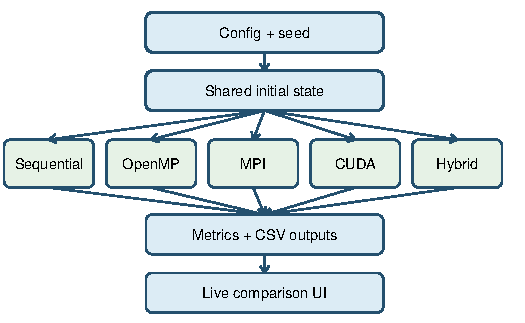
\includegraphics[width=\columnwidth]{figures/architecture.pdf}\caption{Implemented component and output workflow.}\label{fig:architecture}\end{figure}
Sequential CPU is the reference. OpenMP divides updates over threads. MPI assigns contiguous pedestrian ID ranges to ranks; each rank holds the full current state and \texttt{Allgatherv} assembles next state after every step. This is ID partitioning, not spatial decomposition. CUDA launches a pedestrian-parallel kernel with configurable block size. Hybrid assigns ID ranges to MPI ranks, runs the CUDA updater for each range, and uses OpenMP and MPI reduction for metrics. All ranks share one physical GPU \cite{openmp,mpi,cuda}.

\section{Experimental Method}
Measurements used a Windows 11 laptop with Intel Core i7-12650H (10 physical cores, 16 logical processors), approximately 16 GiB RAM, and one GeForce RTX 3050 Laptop GPU (4 GiB), with CUDA Toolkit 13.1, Microsoft MPI, and MSVC. Seed 42 initialized every case. A scaling matrix tested 500, 1,000, 2,000, and 5,000 agents for 100 steps in a 100$\times$70 m room. Three 100-agent exit cases ran 600 steps in a 20$\times$12 m room with 1, 2, and 4 m openings. Each of 35 backend/case combinations received one warmup and five measured runs (175 runs). OpenMP used four threads, MPI two ranks, CUDA blocks of 256, and hybrid two ranks with two OpenMP threads per rank and blocks of 256.

A separate 2,000-agent, 100-step sweep tested 29 configurations with one warmup and five runs each. CPU efficiency is sequential median update time divided by backend median update time and CPU worker count; GPU and hybrid are excluded from this definition. Timing scopes differ: sequential includes next-buffer allocation, MPI includes communication, CUDA includes device allocation and initial upload, and hybrid includes per-step transfer and communication but excludes device allocation. CSV writing and metric sampling are excluded. Cross-backend ratios are indicative local comparisons rather than equivalent end-to-end latency.

Implementation correctness is numerical agreement with sequential, not accuracy against measured human trajectories. Response time is median movement time; movement throughput is steps divided by median seconds. Peak RAM/VRAM and user satisfaction were not measured, so no values are claimed.

\section{Validation and Performance}
All six CTest cases passed. Wide-exit, narrow-exit, and obstacle scenarios agreed on exit counts and active states. Hybrid position and velocity were within 0.001 absolute tolerance over 6,100 saved snapshot rows per scenario; maximum position difference was 0.0002651 m in the narrow-exit case. Summary risk categories and counts agreed, with floating differences at most 0.001. CPU/GPU rounding can place one agent in an adjacent grid cell near a boundary.

Fig.~\ref{fig:runtime} and Table~\ref{tab:runtime} show scaling. At 5,000 agents, indicative ratios to sequential are 3.03$\times$ OpenMP, 1.98$\times$ MPI, 20.54$\times$ CUDA, and 10.00$\times$ hybrid. Movement throughput there is 35.2 steps/s sequential and 722.9 steps/s CUDA. At 500 agents, sequential beats both GPU pathways because setup and communication overhead matter. No agent exited in the short 100-step scaling runs.
\begin{figure}[t]\centering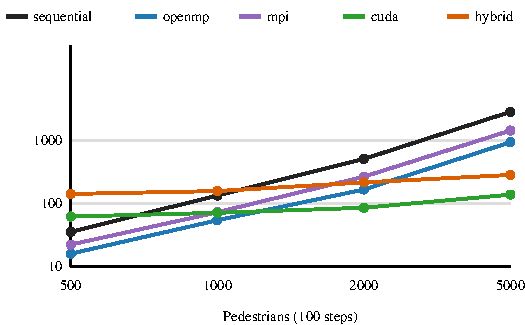
\includegraphics[width=\columnwidth]{figures/runtime.pdf}\caption{Median reported movement time for 100-step scaling cases (log vertical axis; five runs per point).}\label{fig:runtime}\end{figure}
\begin{table}[t]\caption{Median reported movement time (ms)}\label{tab:runtime}\centering\footnotesize
\begin{tabular}{rrrrrr}\toprule Agents&Seq.&OMP&MPI&CUDA&Hybrid\\\midrule
500&35.6&16.1&22.4&62.2&142.0\\1000&134.3&54.4&72.9&71.4&157.9\\
2000&508.9&166.9&266.9&85.9&216.5\\5000&2841.5&938.4&1436.0&138.3&284.2\\\bottomrule\end{tabular}\end{table}

Table~\ref{tab:cpu} reports CPU update speedup and efficiency. OpenMP improved through four threads, whereas eight threads increased update time. CUDA block medians at 128, 256, and 512 threads were 75.10, 76.99, and 81.57 ms; their interquartile ranges overlap. With blocks of 256 and two OpenMP threads per rank, hybrid took 55.02, 166.84, and 342.09 ms at one, two, and four ranks. Sharing one GPU added transfer and communication overhead.
\begin{table}[t]\caption{Fixed 2,000-agent CPU sweep; five-run medians}\label{tab:cpu}\centering\footnotesize
\begin{tabular}{lrrrr}\toprule Path&Workers&Update ms&Speedup&Efficiency\\\midrule
Sequential&1&491.04&1.00&1.00\\OpenMP&2&246.86&1.99&0.99\\OpenMP&4&130.14&3.77&0.94\\OpenMP&8&146.88&3.34&0.42\\MPI&2&247.27&1.99&0.99\\MPI&4&150.23&3.27&0.82\\\bottomrule\end{tabular}\end{table}

\section{Exit-Width and Congestion Results}
The risk study ran 100 and 200 pedestrians for 600 steps (12 s) in a 20$\times$12 m room at exit widths 1, 2, and 4 m. Metrics were saved every 0.2 s; congestion duration accumulated every 0.02 s step. All five backends agreed on recorded categories and integer counts in 30 scenario/backend summaries, with floating differences at most 0.001. Table~\ref{tab:risk} shows sequential results.
\begin{table}[t]\caption{Sequential 12 s exit results}\label{tab:risk}\centering\footnotesize
\begin{tabular}{rrrrrl}\toprule People&Exit m&Exited&Peak density&Congest. s&Risk\\\midrule
100&1&26&6&6.34&high\\100&2&44&4&2.58&high\\100&4&52&3&2.06&medium\\
200&1&46&7&6.92&high\\200&2&76&6&6.10&high\\200&4&97&5&5.34&high\\\bottomrule\end{tabular}\end{table}
Peak density is the maximum recorded sample in people/m$^2$; congestion is maximum cell cumulative duration. For both crowds, wider openings increased exits and reduced peak density and cumulative congestion. At 100 agents the 4 m case reached only medium, whereas all three 200-agent cases reached high. These observations use one seed and chosen thresholds, not real evacuation probabilities.

\section{Limitations and Security}
The model omits contact friction, behavior changes, route choice, and empirical calibration. Pedestrian contact is soft; no pressure or injury outcome validates risk labels. MPI splits IDs, and hybrid tests used one GPU and one machine. Repeated seeds, independent hardware, measured trajectories, and uniform end-to-end timing are needed for generality. Configuration validation rejects unknown or duplicate keys and invalid geometry. Before sharing the interface beyond a trusted local machine, its server and output paths need access control and further input hardening. Risk labels must remain visibly simulated indicators.

\section{Future Work}
Next steps are trajectory calibration, repeated-seed sensitivity, end-to-end timing, and peak CPU/GPU memory profiling. Spatial MPI partitioning could reduce state replication; multi-GPU experiments are required before claiming distributed GPU scaling. Usability needs a defined task and participants before reporting satisfaction.

\section{Conclusion}
Five backends reproduced exit outcomes and summary indicators within validation tolerance. CUDA reported 138.34 ms for the 5,000-agent, 100-step case versus 2,841.54 ms sequential on this machine; four-thread OpenMP reached 3.77$\times$ CPU update speedup in the fixed sweep. Wider openings yielded more exits and less recorded congestion. The simulator supports controlled implementation comparison and exploratory bottleneck analysis within its stated limits.

\begin{thebibliography}{9}
\bibitem{helbing1995} D. Helbing and P. Moln\'ar, ``Social force model for pedestrian dynamics,'' \emph{Phys. Rev. E}, vol. 51, pp. 4282--4286, 1995, doi: 10.1103/PhysRevE.51.4282.
\bibitem{helbing2000} D. Helbing, I. Farkas, and T. Vicsek, ``Simulating dynamical features of escape panic,'' \emph{Nature}, vol. 407, pp. 487--490, 2000, doi: 10.1038/35035023.
\bibitem{helbing2007} D. Helbing, A. Johansson, and H. Zein Al-Abideen, ``Dynamics of crowd disasters: An empirical study,'' \emph{Phys. Rev. E}, vol. 75, 046109, 2007, doi: 10.1103/PhysRevE.75.046109.
\bibitem{openmp} OpenMP Architecture Review Board, \emph{OpenMP Application Programming Interface, Version 5.2}, 2021. [Online]. Available: https://www.openmp.org/specifications/
\bibitem{mpi} MPI Forum, \emph{MPI: A Message-Passing Interface Standard, Version 4.1}, 2023. [Online]. Available: https://www.mpi-forum.org/docs/mpi-4.1/
\bibitem{cuda} NVIDIA, \emph{CUDA Programming Guide}. [Online]. Available: https://docs.nvidia.com/cuda/cuda-programming-guide/
\bibitem{grandison2017} A. Grandison, Y. Cavanagh, P. J. Lawrence, and E. R. Galea, ``Increasing the simulation performance of large-scale evacuations using parallel computing techniques based on domain decomposition,'' \emph{Fire Technology}, vol. 53, pp. 1399--1438, 2017, doi: 10.1007/s10694-016-0645-8.
\bibitem{choi2025} C.-H. Choi \emph{et al.}, ``Prediction and prevention of crowd-crush accidents using crowd-density simulation based on unity engine,'' \emph{Discover Applied Sciences}, vol. 7, art. 33, 2025, doi: 10.1007/s42452-024-06451-7.
\bibitem{shigenaka2024} S. Shigenaka, S. Takami, Y. Tanigaki, S. Watanabe, and M. Onishi, ``MAS-Bench: a benchmarking for parameter calibration of multi-agent crowd simulation,'' \emph{Journal of Computational Social Science}, vol. 7, pp. 2121--2145, 2024, doi: 10.1007/s42001-024-00302-6.
\end{thebibliography}
\end{document}
